\documentclass[aspectratio=169]{beamer}
%\usepackage{ngerman}
\usepackage[utf8]{inputenc} 

\usepackage{listings}
\usepackage{color}

\usetheme{Warsaw}  %% Themenwahl


\usepackage{pgfpages}
%\setbeameroption{show notes}
%\setbeameroption{show notes on second screen=right}
 
\title{All about class loading!}
\author{Felix Becker}
\date{\today}
\institute{Amsterdam.scala}


\titlegraphic{
 % 
\includegraphics[width=2cm]{assets/amsterdam-scala.png}\hspace*{4.75cm}~%
   
\includegraphics[width=2cm]{assets/amsterdam-scala.png}
}



\definecolor{javared}{rgb}{0.6,0,0} % for strings
\definecolor{javagreen}{rgb}{0.25,0.5,0.35} % comments
\definecolor{javapurple}{rgb}{0.5,0,0.35} % keywords
\definecolor{javadocblue}{rgb}{0.25,0.35,0.75} % javadoc
 
 \lstset{language=Java,
 basicstyle=\tiny,
 keywordstyle=\color{javapurple}\bfseries,
 stringstyle=\color{javared},
 commentstyle=\color{javagreen},
 morecomment=[s][\color{javadocblue}]{/**}{*/},
 numbers=left,
 numberstyle=\tiny\color{black},
 stepnumber=1,
 numbersep=10pt,
 tabsize=2,
 xleftmargin=1cm,
 showspaces=false,
 showstringspaces=false}


 
\begin{document}
\maketitle


\begin{frame}
	\frametitle{Contents}
	\tableofcontents
\end{frame}


% do i need this in amsterdam?
\begin{frame}
	\frametitle{Motivation}
	\begin{itemize}
		\item{Scala runs on the JVM (which is a good thing!)}
		\item{You can solve complex classpath problems with knowledge about class loading}
		\item{Deep knowledge of the JVM always enables you to do cool things (e.g. byte code instrumentation)}
		\item{Knowledge about JVM byte code requires knowledge about class loading techniques}
	\end{itemize}
\end{frame}

\section{Class Loading basics}

\begin{frame}
	\frametitle{Task of a class loader?}
	\begin{itemize}
		\item{Load classes and resources from different sources}
		\item{Distinction between data source and application, application only must use the class loader (platform independency)}
		\item{Classes are being loaded in the JVM byte code format}
		\item{Resources can be any data (e.g. a file from the file system of from a web service call)}
	\end{itemize}
\end{frame}

\subsection{Class startup life cycle}

\begin{frame}
	\frametitle{Startup life cycle of a Java class (JVM spec §12.1.2)}
	\begin{enumerate}
		\item{Loading §12.2.1}
			\begin{itemize}
				\item{Load the bytecode into the JVM using the class loader}
			\end{itemize}
		\item{Verify §12.3.1}
			\begin{itemize}
				\item{Validation of the class structure and data (Opcodes valid, branch instructions check, signature check, ...)}
			\end{itemize}
		\item{Prepare §12.3.2}
			\begin{itemize}
				\item{Storage allocation, initialization of static fields (default values, no static initializer)}
			\end{itemize}
		\item{(Resolve §12.3.3)}
			\begin{itemize}
				\item{Optional step: symbolic link resolution}
			\end{itemize}
		\item{Initialization §12.4.1}
			\begin{itemize}
				\item{Call to static initializers, initialization of static fields}
			\end{itemize}
	\end{enumerate}
\end{frame}

\begin{frame}
	\frametitle{Initialization}
	Initialization of a class is the first ''active'' code execution of class code (if static fields / initializers exist). Initialization happens the first time (only once), when:
	\begin{itemize}
		\item{An instance of the class is being created}
		\item{A static method of the class is being invoked}
		\item{Static variables are read / written}
	\end{itemize}

	Initialization of a class forces the initialization of all super classes (does not happen for interface) % TODO still valid in java 8?
	\begin{block}{Initialization of a class is thread safe - safe way to create singletons!}
		The initialization is secured by a jvm internal initialization lock. The jvm guarantees, that the initialization of a class happens only once.
	\end{block}
\end{frame}

\subsection{ClassLoader delegation model}

\begin{frame}
	\frametitle{Default class loader JVM 8 (Oracle)}
	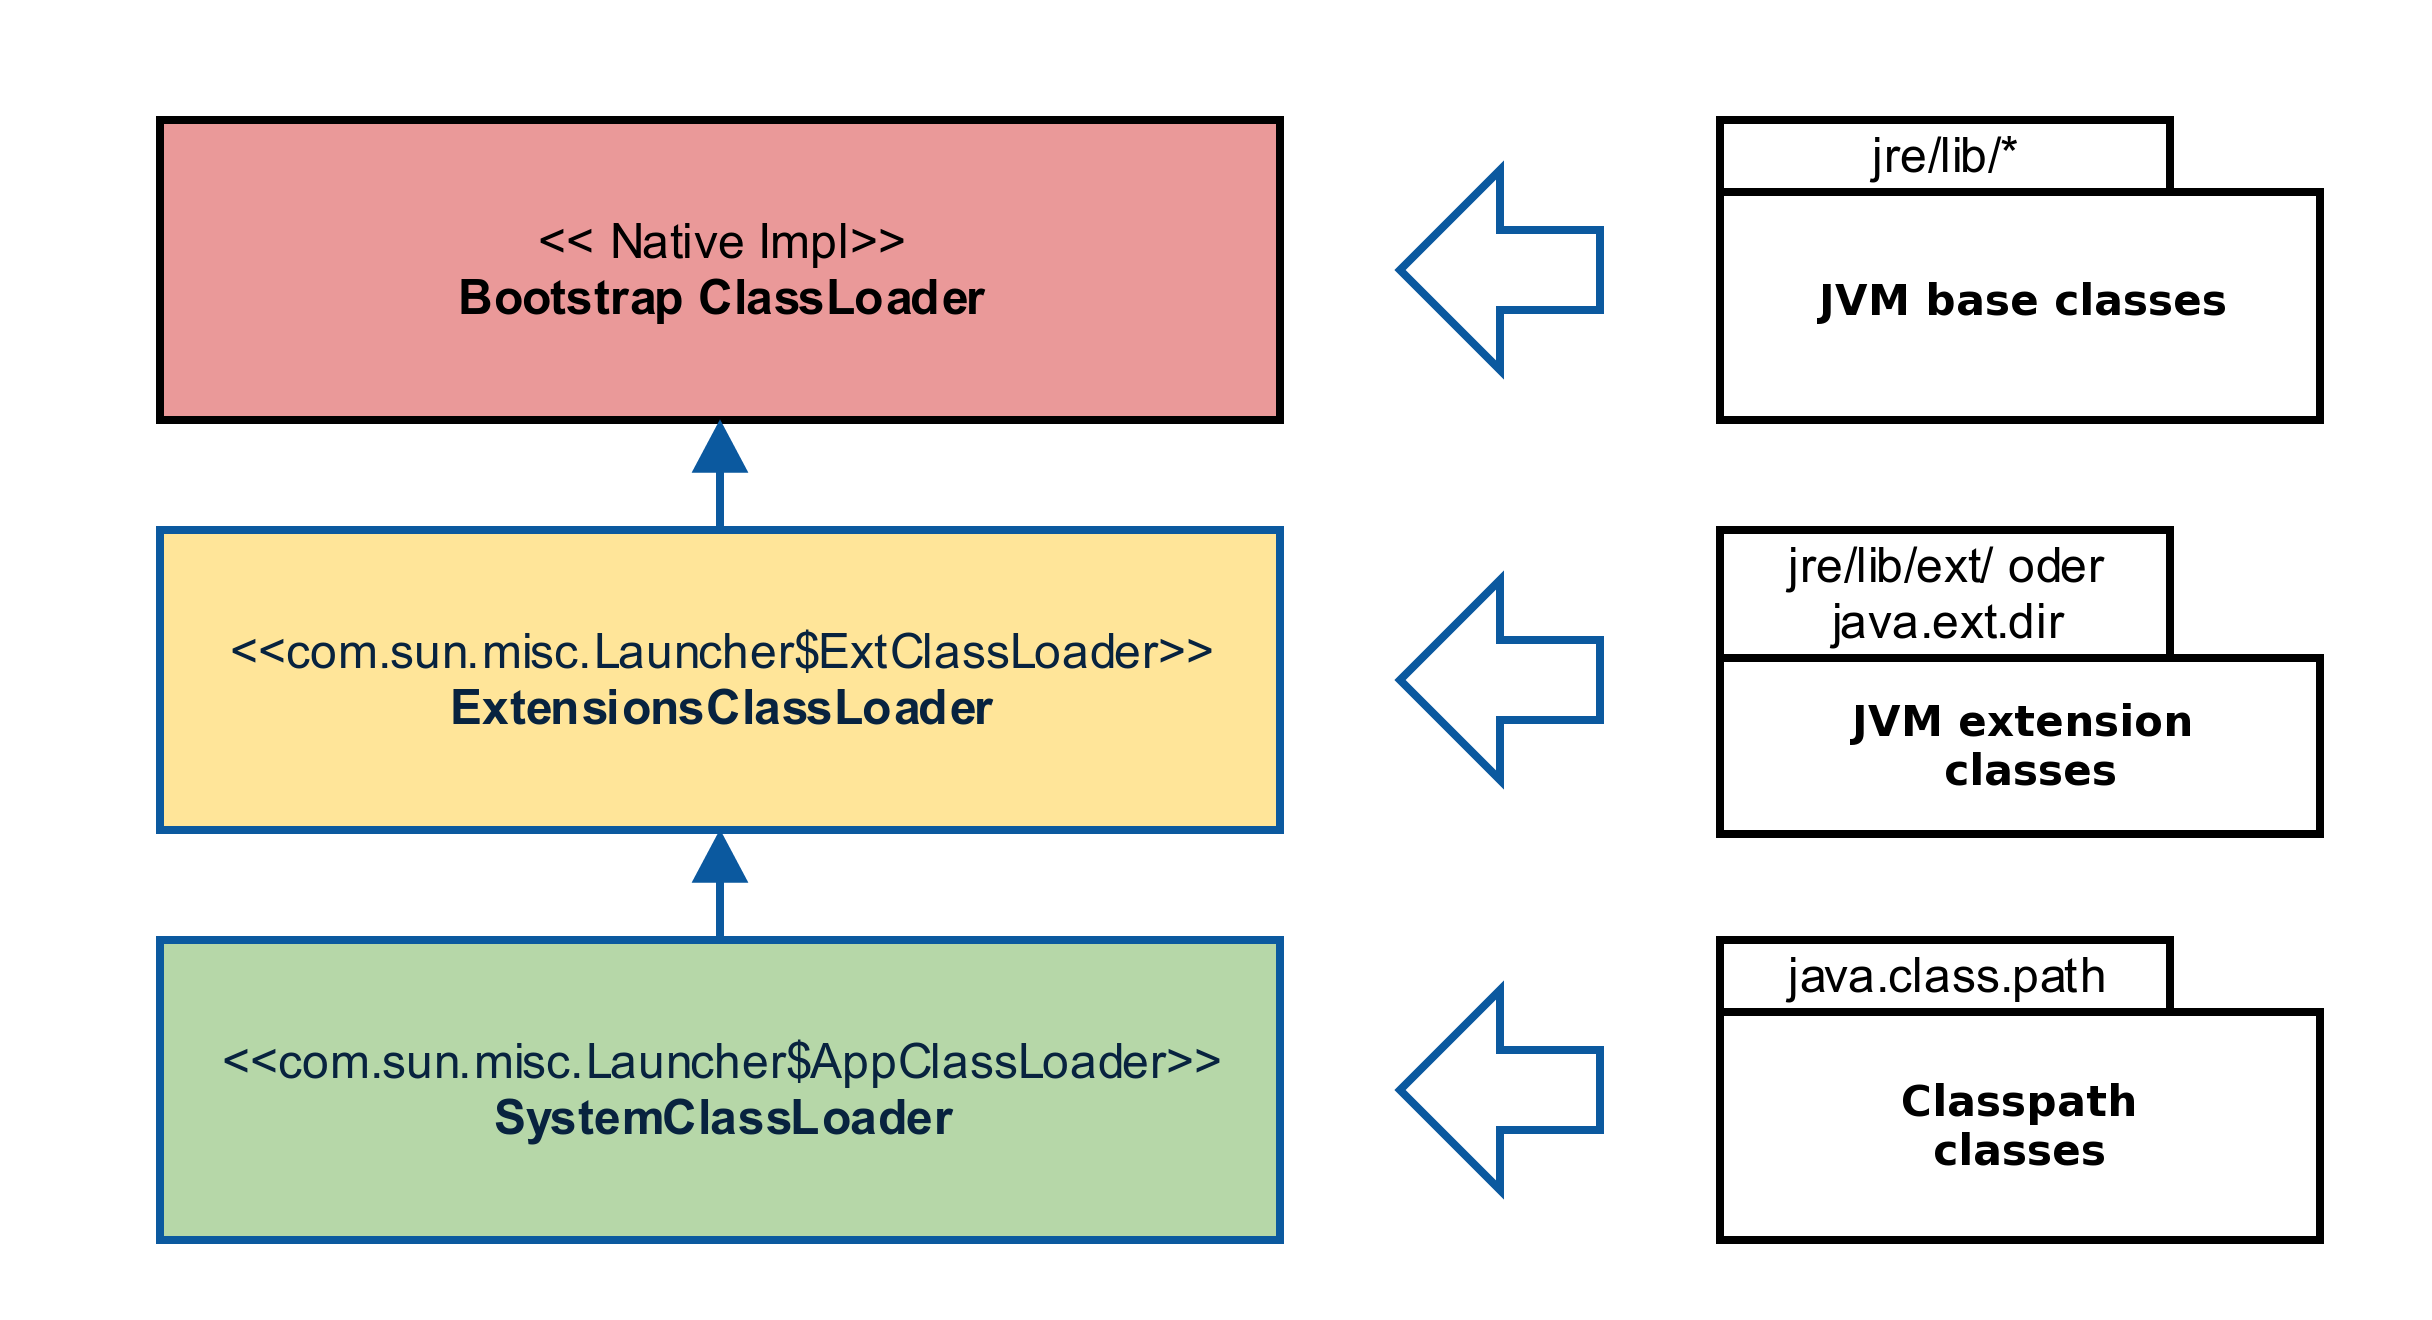
\includegraphics[scale=0.1]{assets/classloader-hierachie.png} 
\end{frame}

\begin{frame}
	\frametitle{Bootstrap class loader}
	\begin{columns}[T] 
		\begin{column}{.46\textwidth}
			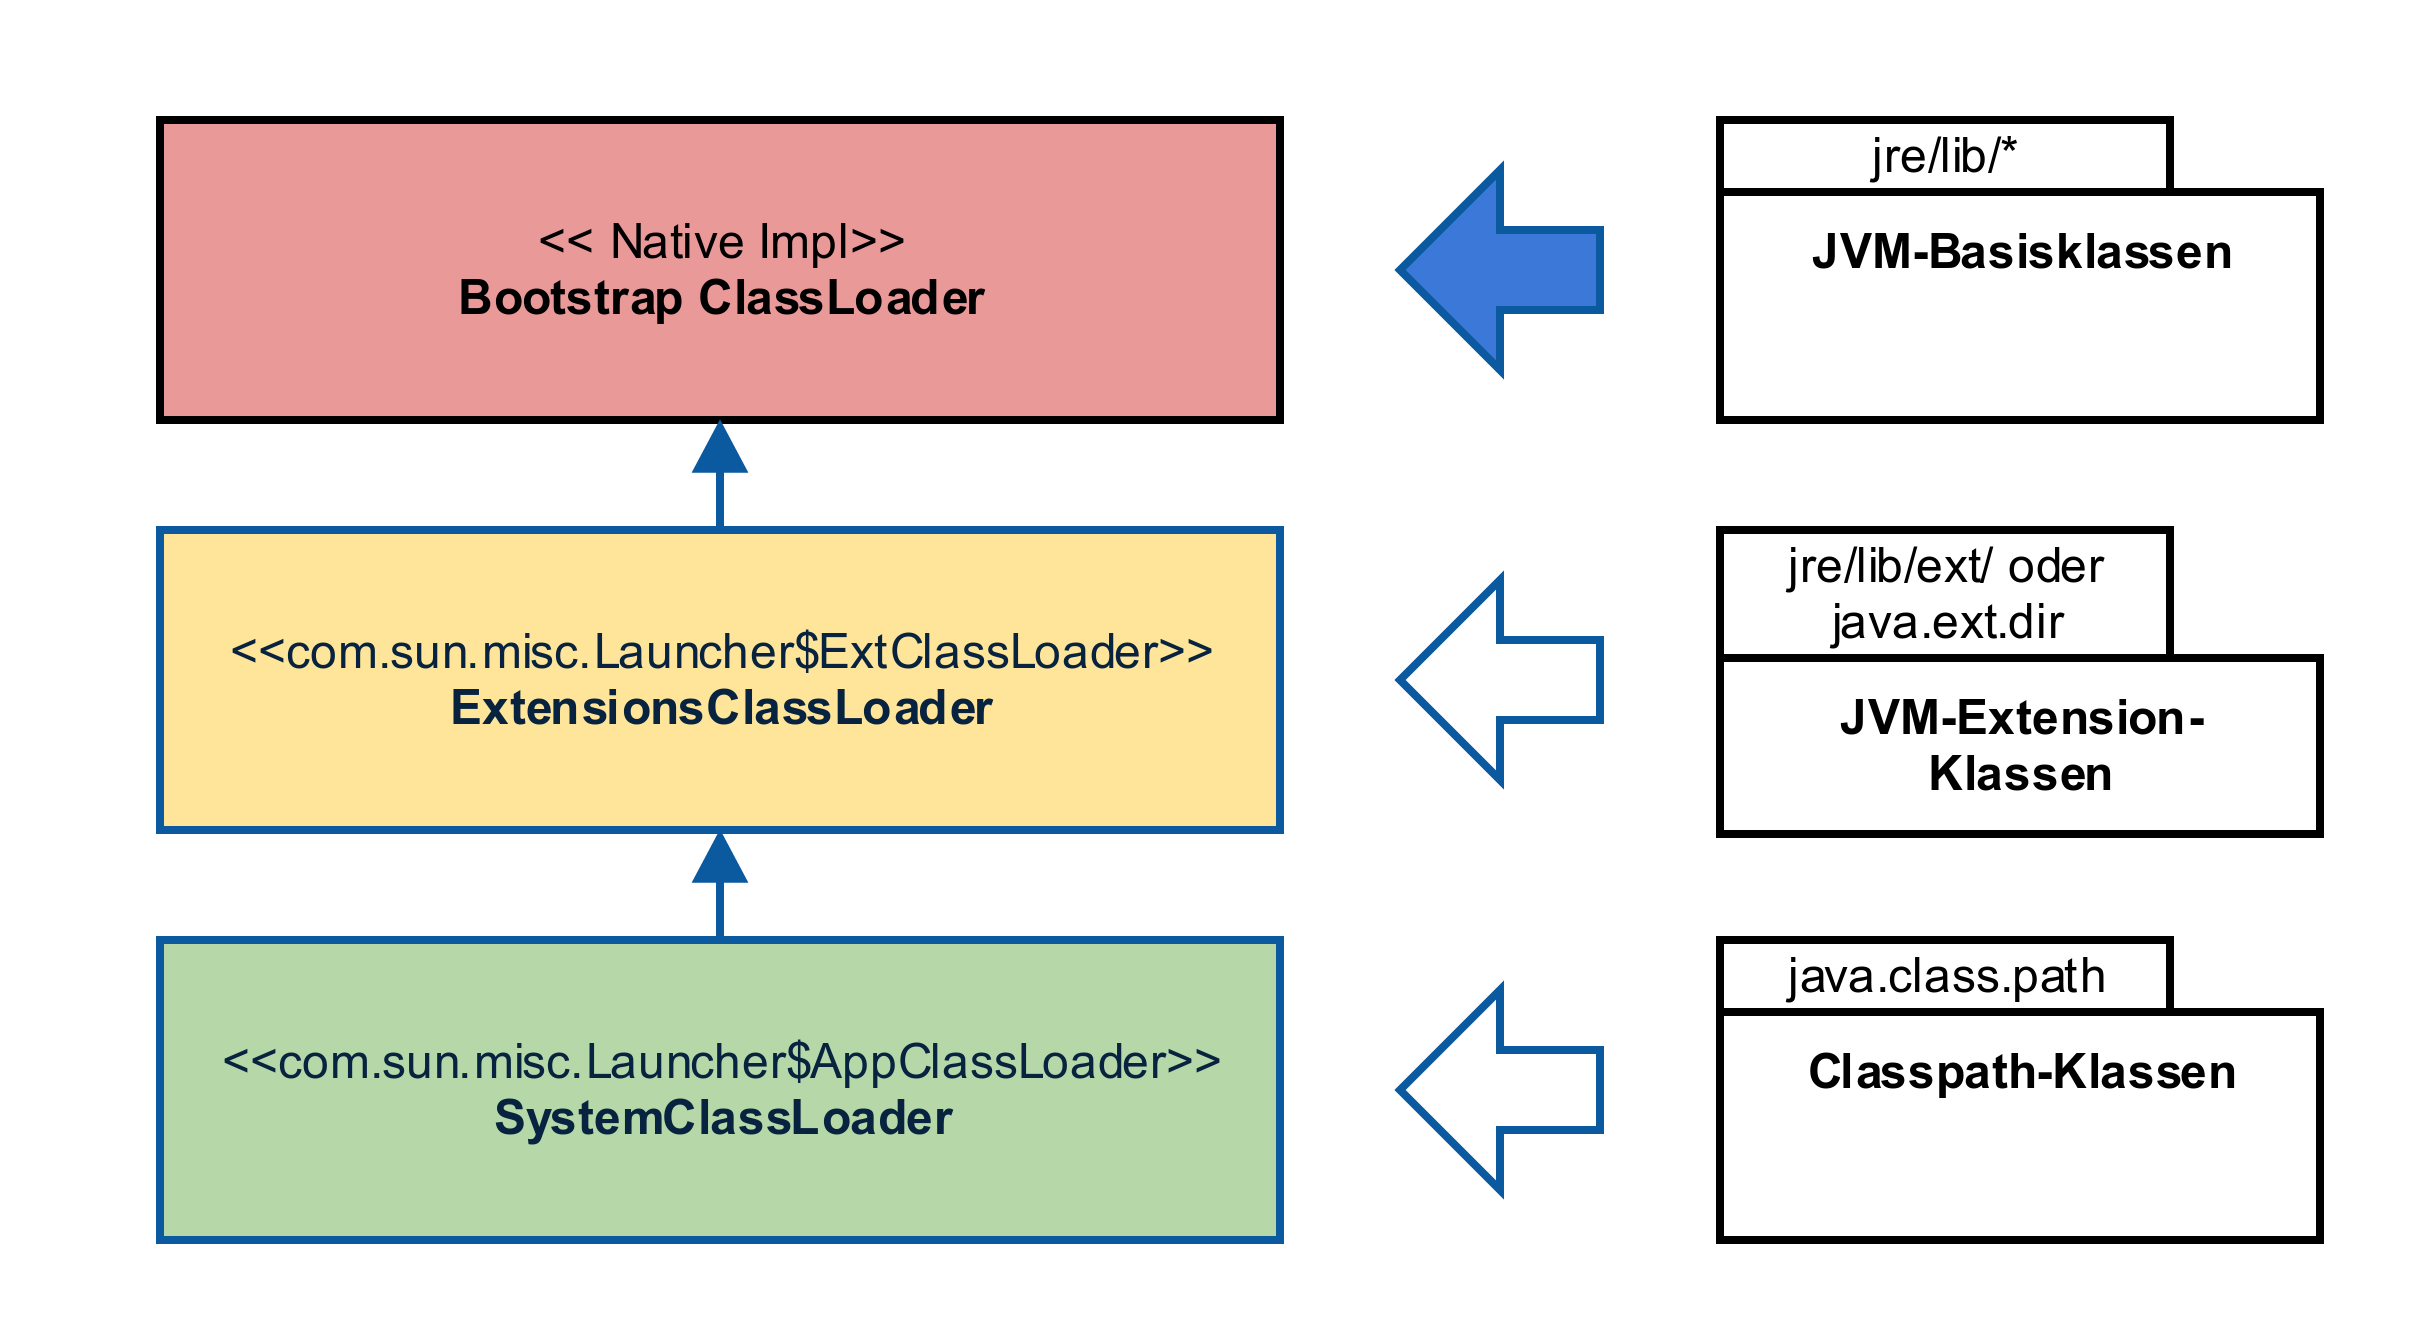
\includegraphics[scale=0.06]{assets/classloader-hierachie-bootstrap-active.png}
		\end{column}
		\hfill
		\begin{column}{.56\textwidth}

		\begin{itemize}
			\item{Loads Java base classes (e.g. java/lang/String)}
			\item{Native implementation}
			\item{java.lang.ClassLoader: private native Class findBootstrapClass}
		\end{itemize}

		\end{column}
	\end{columns}
\end{frame}

\begin{frame}
	\frametitle{Extension class loader}
	\begin{columns}[T] 
		\begin{column}{.46\textwidth}
			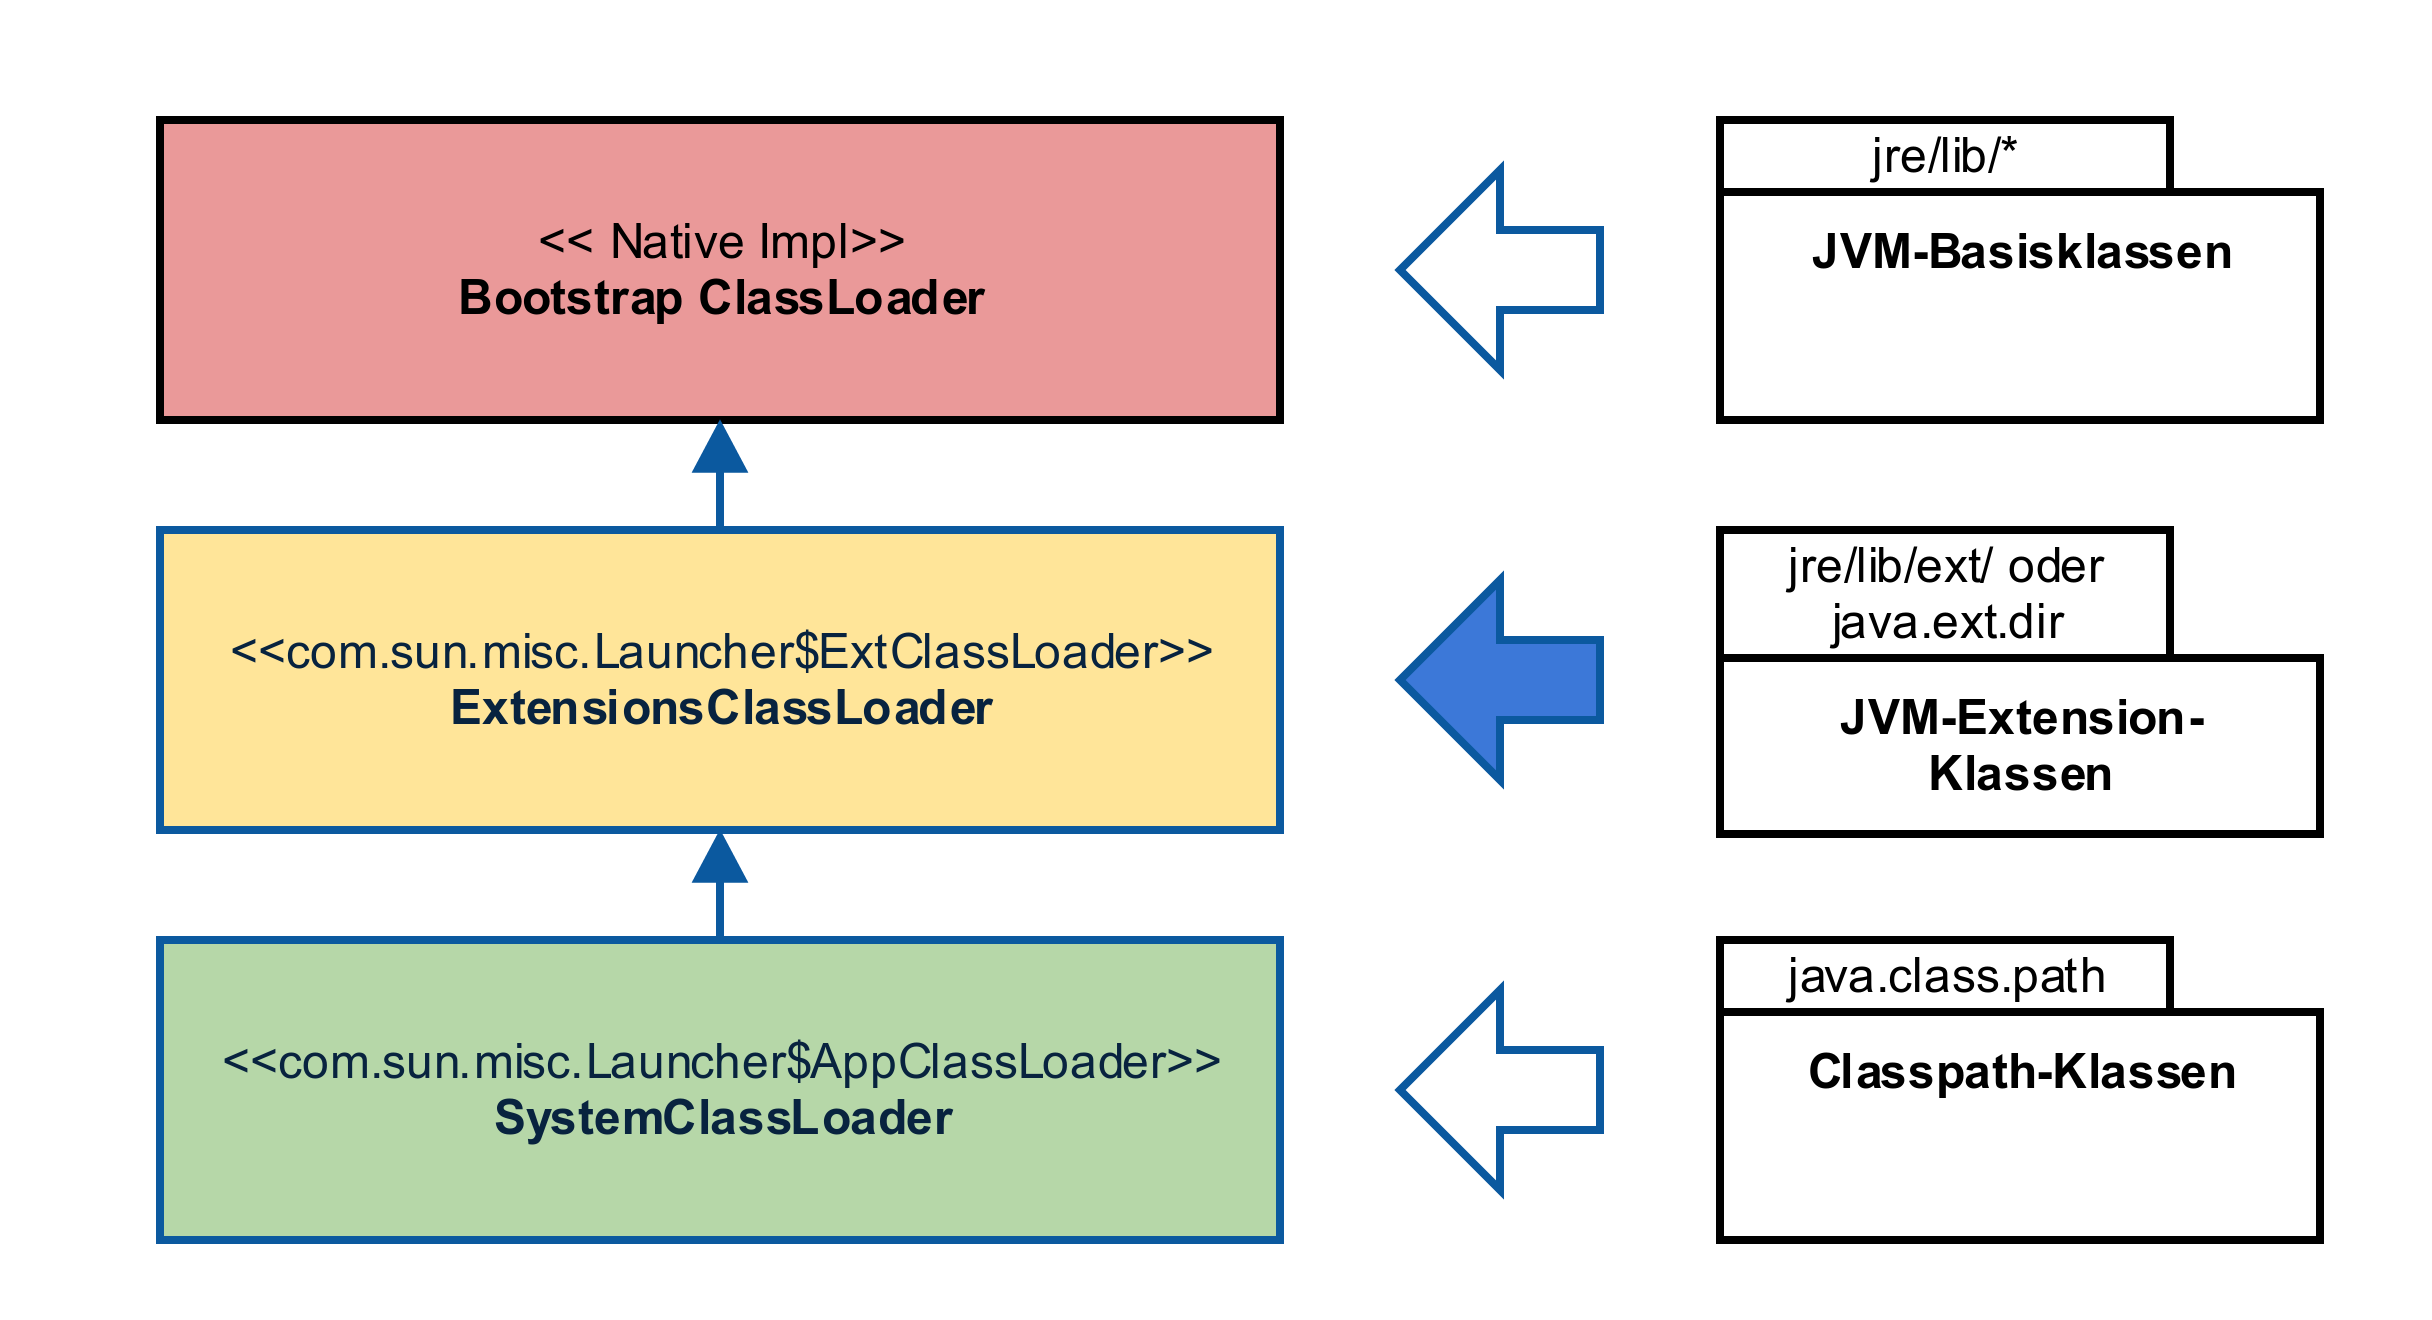
\includegraphics[scale=0.06]{assets/classloader-hierachie-extension-active.png}
		\end{column}
		\hfill
		\begin{column}{.56\textwidth}

		\begin{itemize}
			\item{Loads extension classes}
			\item{Example: com/sun/nio/zipfs/ZipPath}
			\item{Loads classes from jre/lib/ext/ or java.ext.dirs}
			\item{com.sun.misc.Launcher\$ExtClassLoader}
		\end{itemize}
		\end{column}
	\end{columns}
\end{frame}

\begin{frame}
	\frametitle{System class loader}
	\begin{columns}[T] 
	\begin{column}{.46\textwidth}
		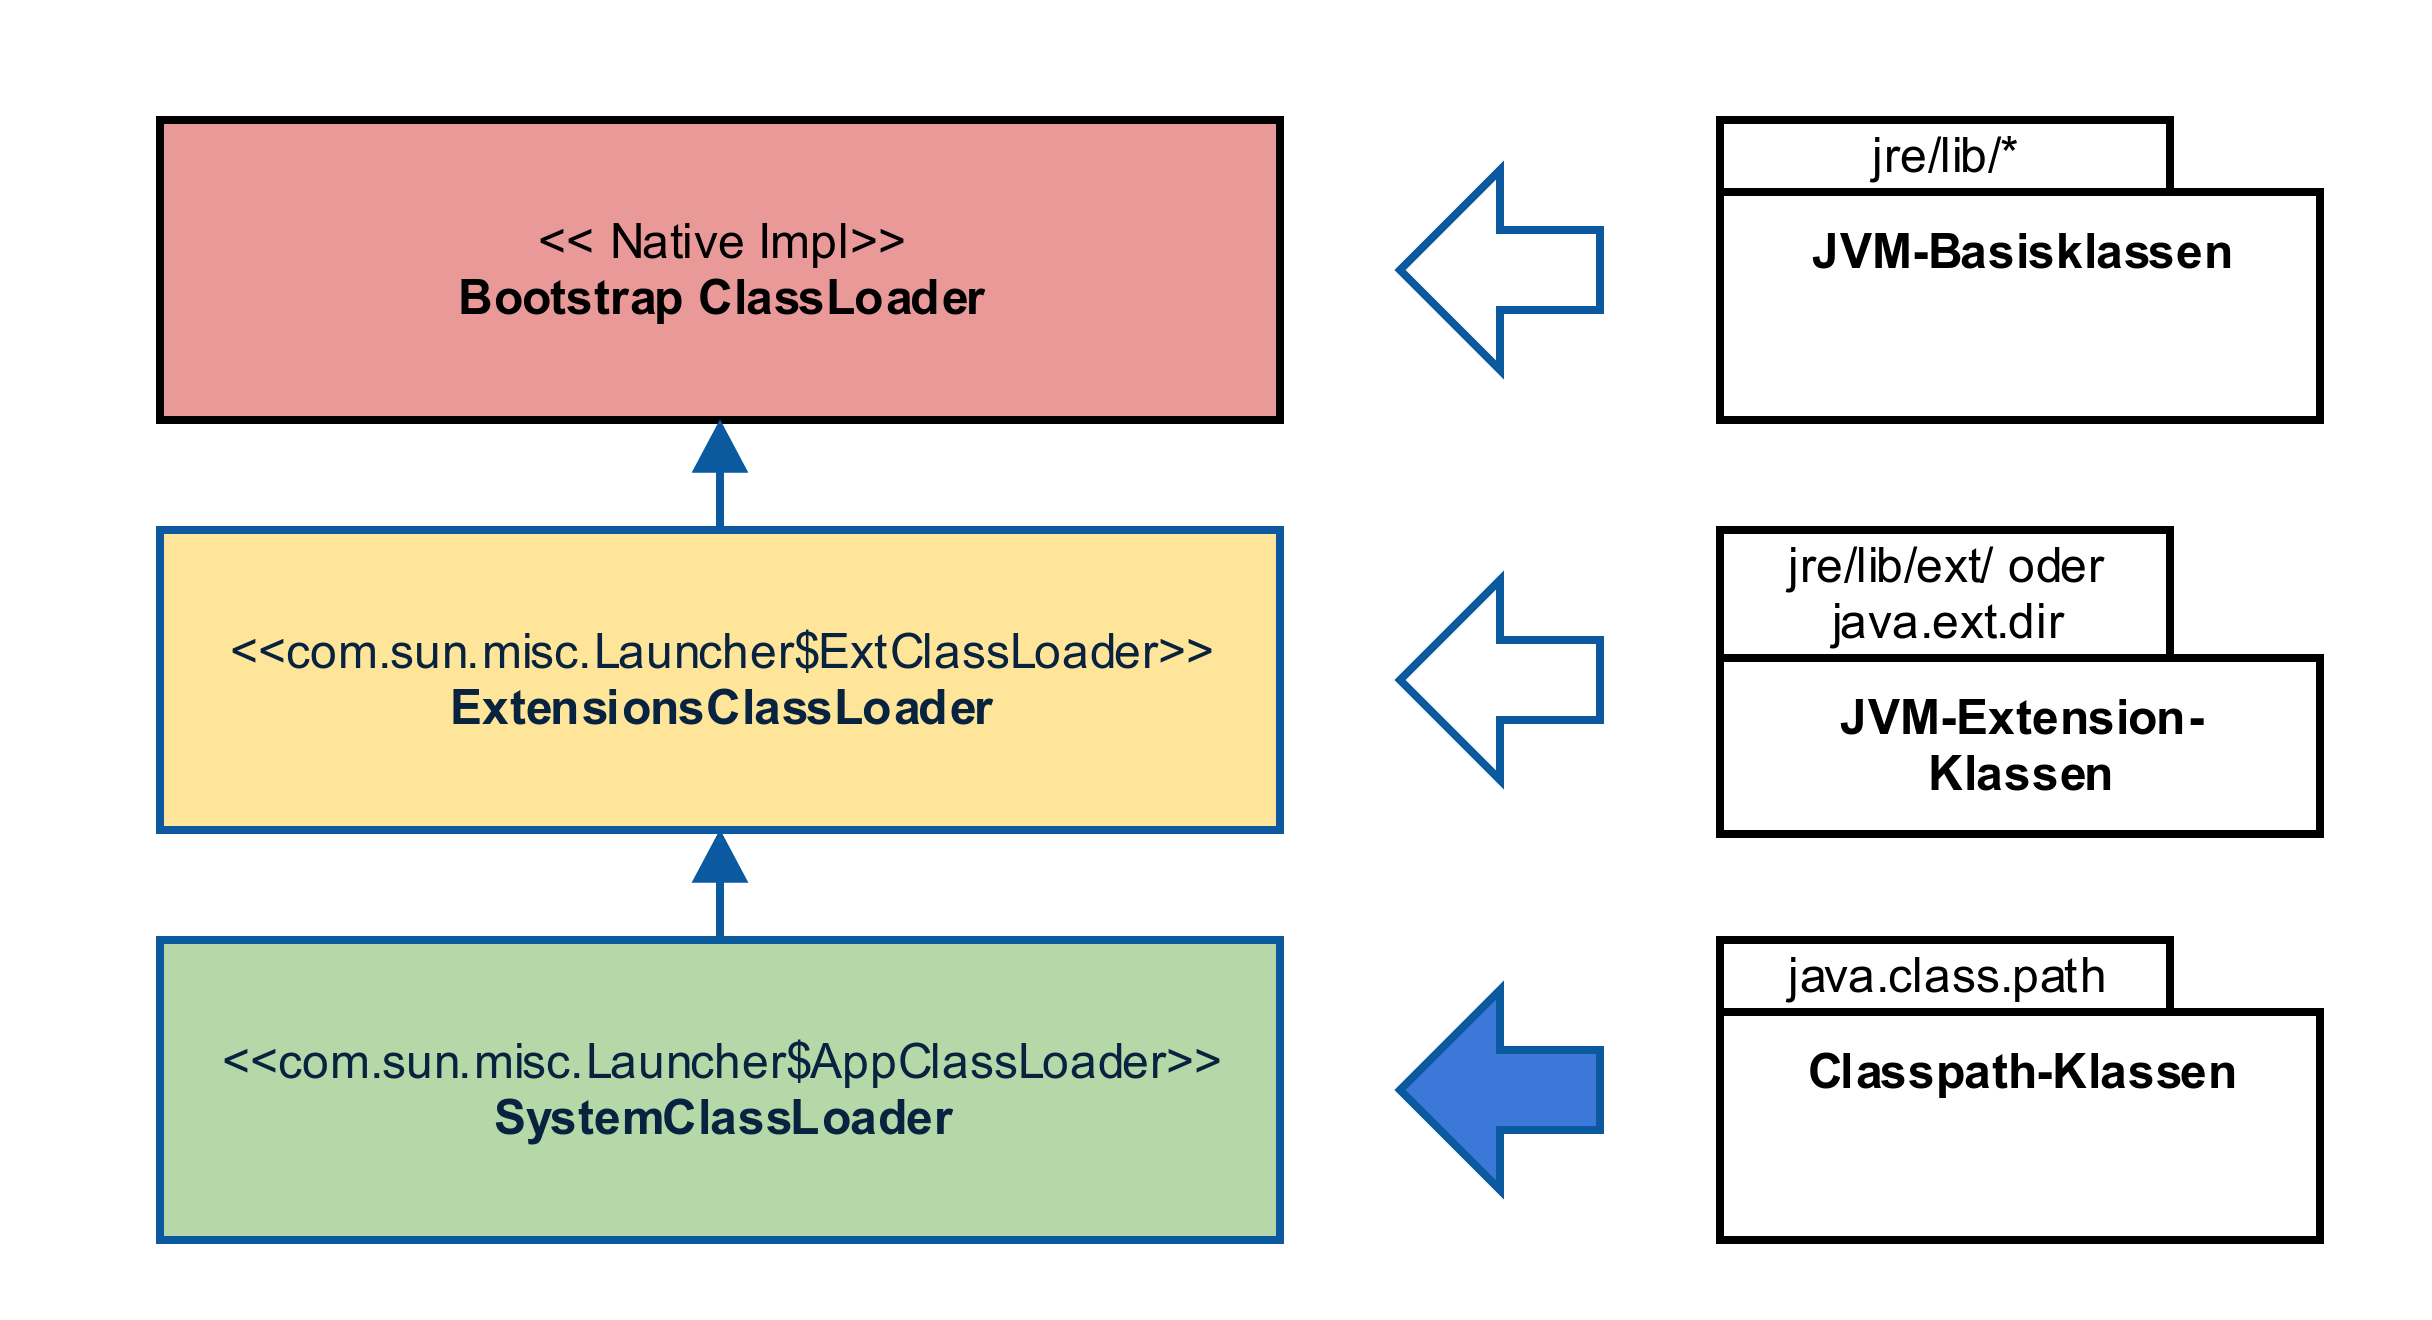
\includegraphics[scale=0.06]{assets/classloader-hierachie-system-active.png}
	\end{column}
	\hfill
	\begin{column}{.56\textwidth}

	\begin{itemize}
		\item{Loads all classes from the java.class.path (java -cp ..)}
		\item{java.class.path (com.sun.misc.Launcher\$AppClassLoader)}
	\end{itemize}

	\end{column}
	\end{columns}
\end{frame}

\section{Class loader implementations}

\begin{frame}
	\frametitle{Important functions}
	\begin{itemize}
		\item{From the applications point of view:}
			\begin{itemize}
				\item{Class.forName(String)}
				\item{Class.getClassLoader()}
				\item{ClassLoader.loadClass(String)}
			\end{itemize}
		\item{Inside the class loader:}
			\begin{itemize}
				\item{findLoadedClass(String)}
				\item{findBootstrapClassOrNull(String)}
				\item{resolveClass}
				\item{defineClass}
			\end{itemize}
	\end{itemize}
\end{frame}

\begin{frame}
	Live-Demo 1: First steps
\end{frame}

\begin{frame}
	\frametitle{ClassLoader.loadClass}
	\begin{columns}[T] 
		\begin{column}{.57\textwidth}
			\lstinputlisting{ClassLoaderLoadClass.java}
		\end{column}
		\hfill
		\begin{column}{.43\textwidth}
			\begin{itemize}
				\item{Class loading ist synchronized in loadClass, too}
				\item{lookup steps:}
				\begin{enumerate}
					\item{findLoadedClass (native)}
					\item{parent / bootstrap lookup}
					\item{findClass}
				\end{enumerate}
				\item{findClass is the function you have to override in your own class loader implementation}
			\end{itemize}
		\end{column}
	\end{columns}
\end{frame}

\begin{frame}
	\frametitle{ClassLoader.resolveClass}
	\lstinputlisting{resolveClass.java}
	\begin{quote}
		\tiny{Loads the class and binds it with resolveClass() - if resolve is true. - (Java ist auch eine Insel)}
	\end{quote}
	\begin{quote}
		\tiny{The variable resolve is a flag to tell the class loader that classes referenced by this class name should be resolved (that is, any referenced class should be loaded as well). - JavaWorld (The basics of Java class loaders)}
	\end{quote}
	\begin{quote}
	\tiny{As I mentioned previously, loading a class can be done partially (without resolution) or completely (with resolution). When we write our version of loadClass, we may need to call resolveClass, depending on the value of the resolve parameter to loadClass. - IBM Developer Works (Understanding the Java ClassLoader)}
	\end{quote}
	Live-Demo 2: resolveClass 
	\pause
	\lstinputlisting{jvm-resolveclass.cpp}
\end{frame}


\begin{frame}[fragile]
	\frametitle{ClassLoader.getResource}
	\begin{columns}[T] 
		\begin{column}{.50\textwidth}
			\lstinputlisting{ClassLoaderGetResource.java}
	\end{column}
	\hfill
	\begin{column}{.50\textwidth}
			\begin{itemize}
				\item{Lookup the resource at the parent / boot strap classloader first}
				\item{findResource is being invoked when the parent / boot strap doesn't provide the resource}
				\item{findResource is the function that you have to override in your own class loader implementation}
			\end{itemize}
		\end{column}
	\end{columns}
\end{frame}

\begin{frame}
	\frametitle{URL-ClassLoader}
	\lstinputlisting{URLClassLoaderFindClass.java}
\end{frame}

\begin{frame}
	Live-Demo 3: URL-ClassLoader
\end{frame}
 
\section{Advanced class loader techniques}


	\subsection{The context class loader \& the web apps}
	\begin{frame}
		\frametitle{WebApp class loader}
		\begin{center}
			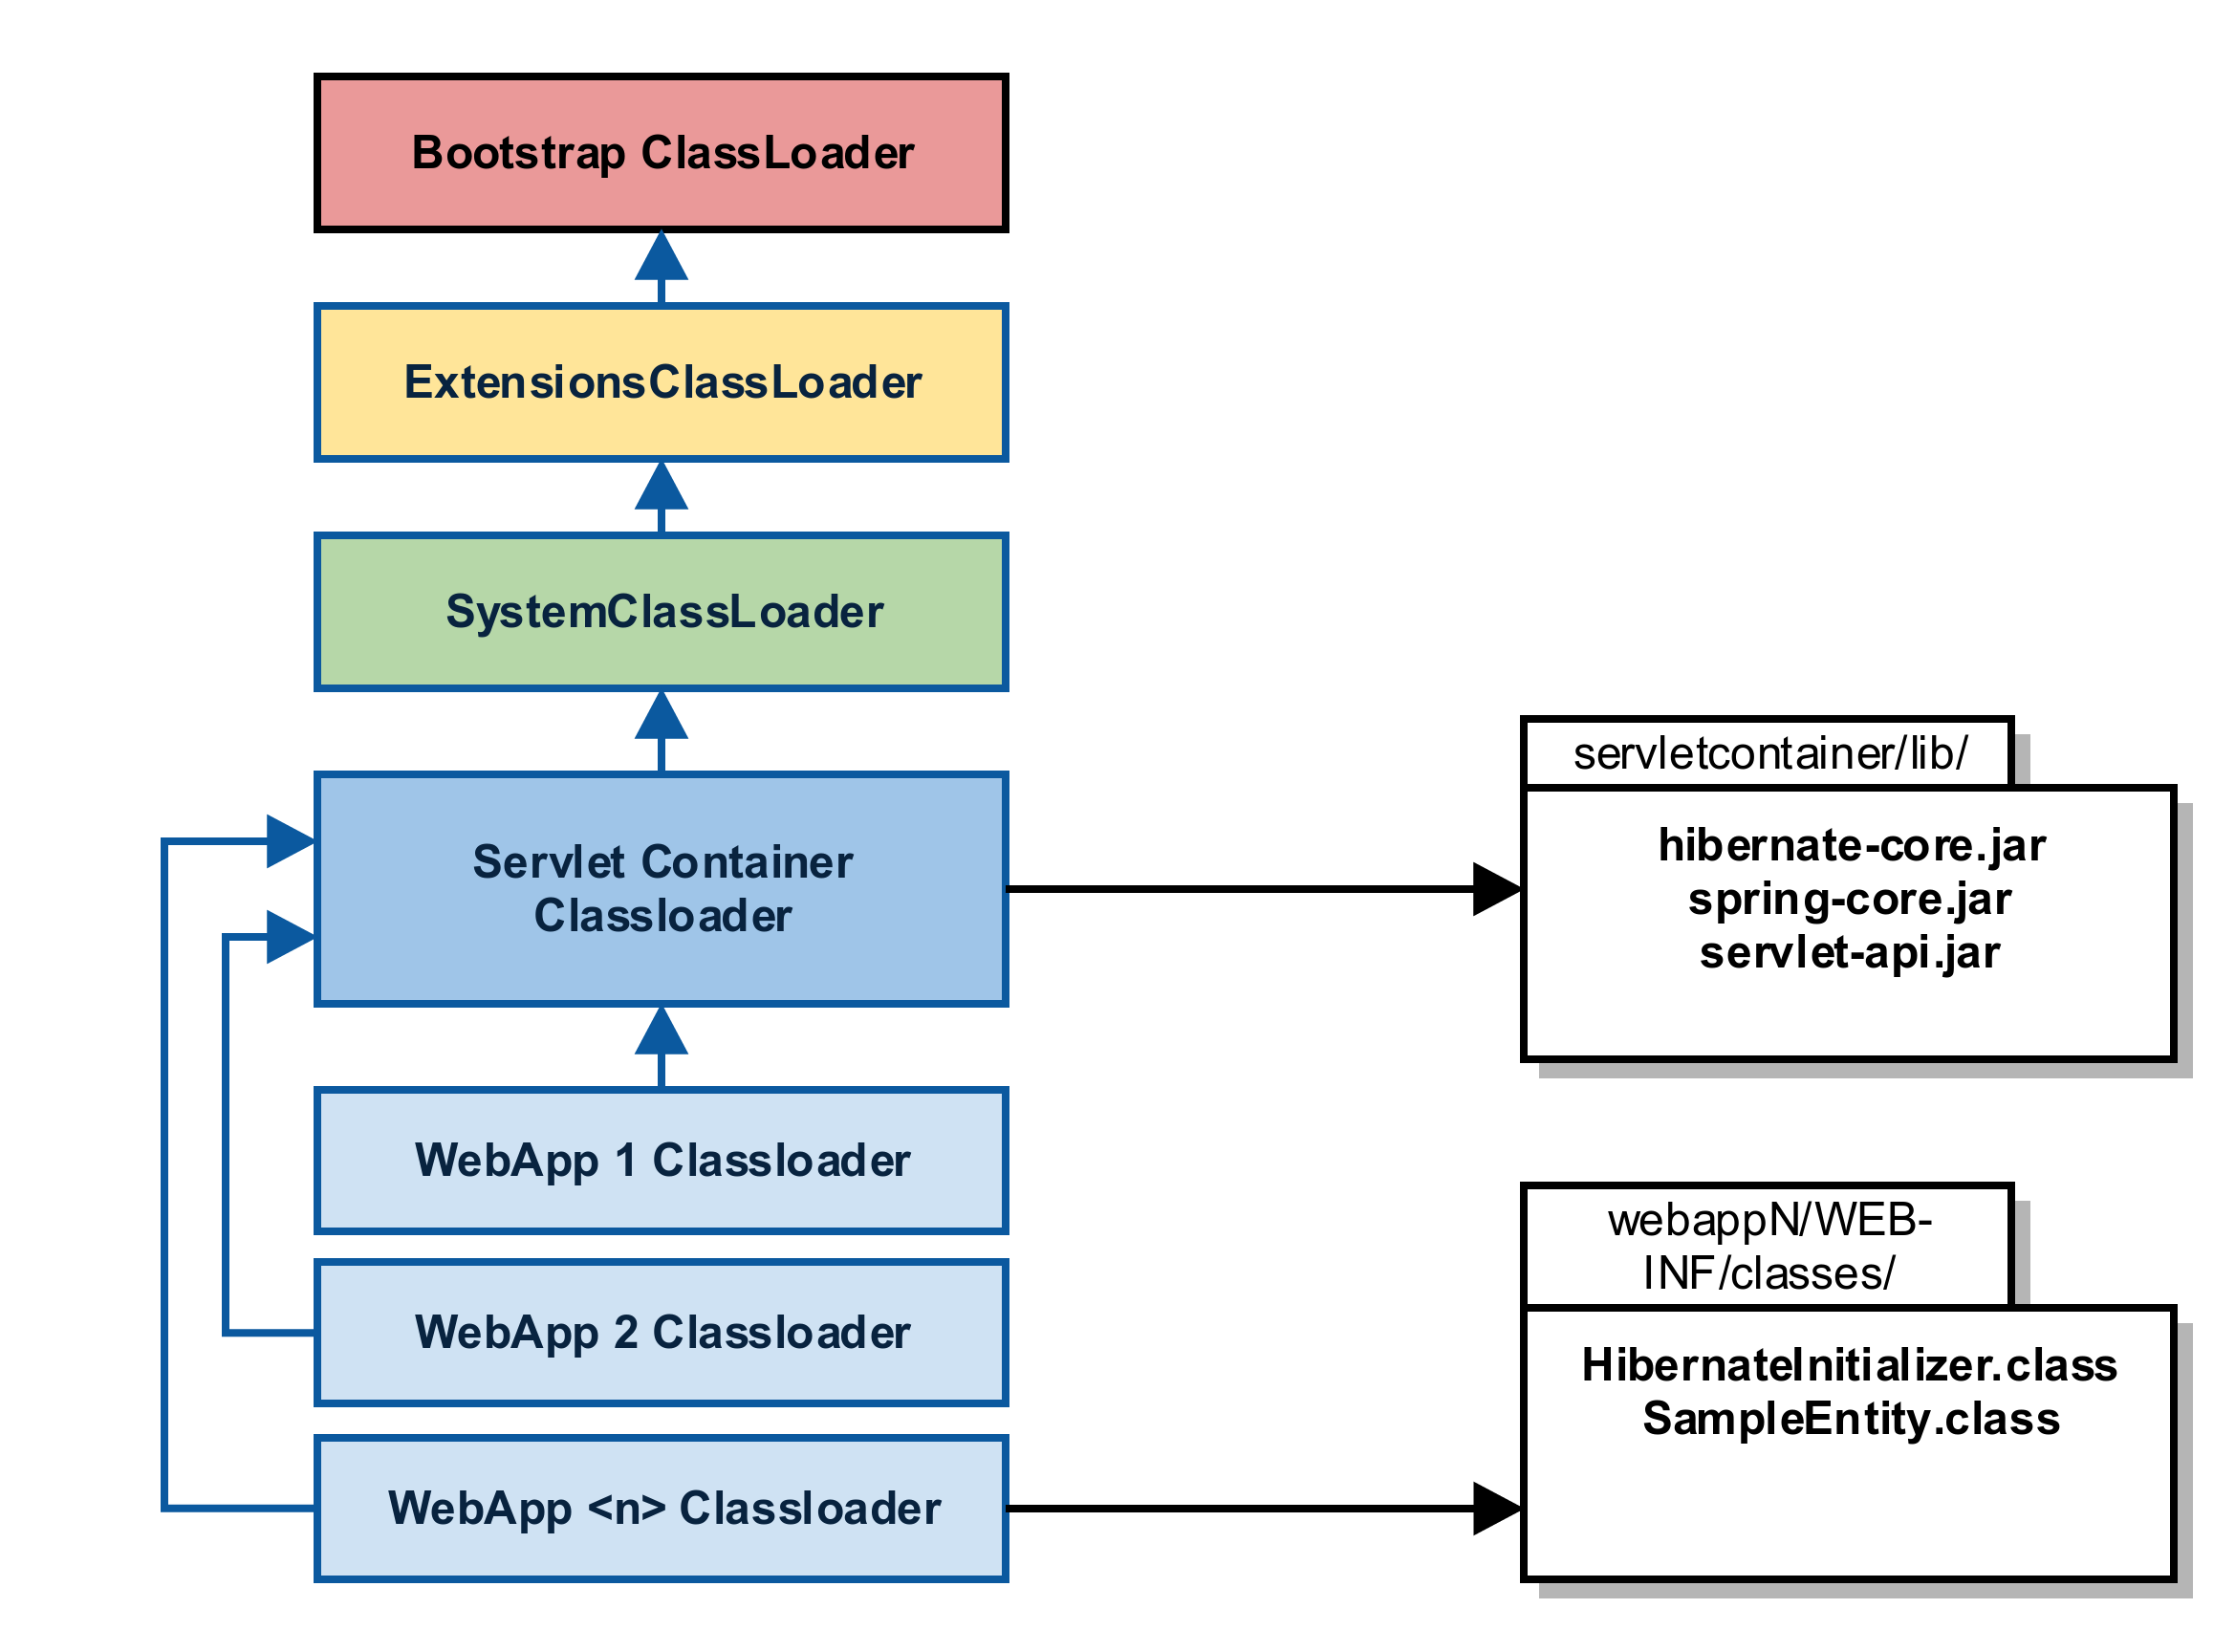
\includegraphics[scale=0.1]{assets/contextclassloader/webappclassloader-1.png} 
		\end{center}
	\end{frame}
	\begin{frame}
		\frametitle{WebApp class loader - context class loader}
		\begin{center}
			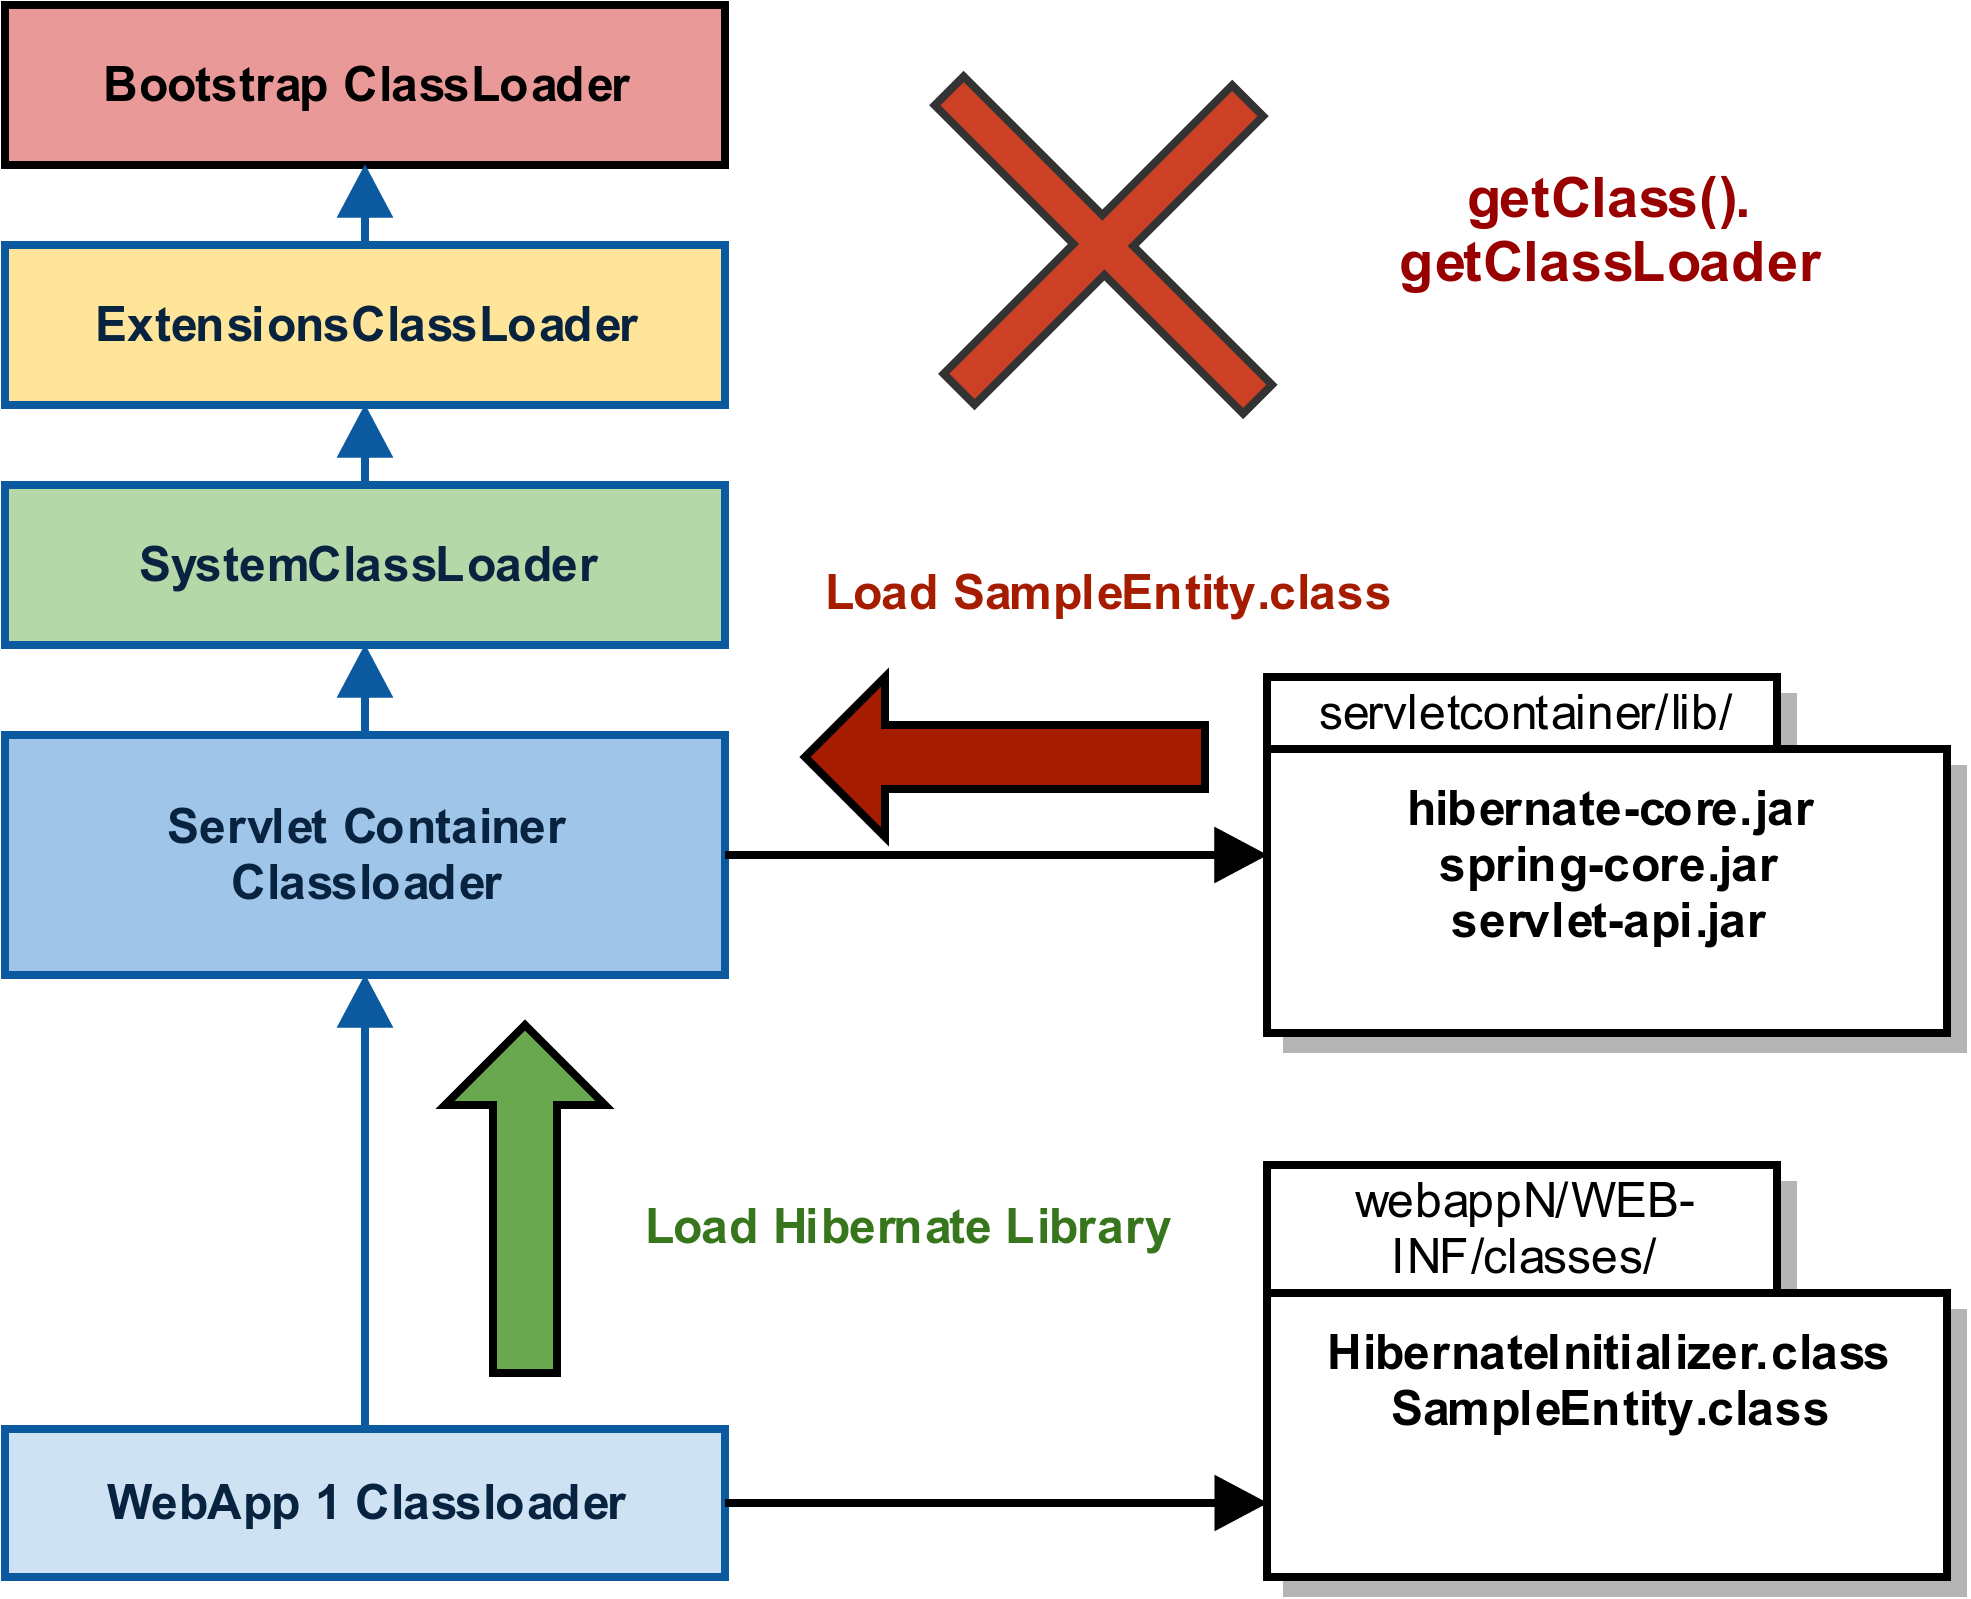
\includegraphics[scale=0.1]{assets/contextclassloader/webappclassloader-2.png} 
		\end{center}
	\end{frame}
	\begin{frame}
		\frametitle{WebApp class loader - context class loader}
		\begin{center}
			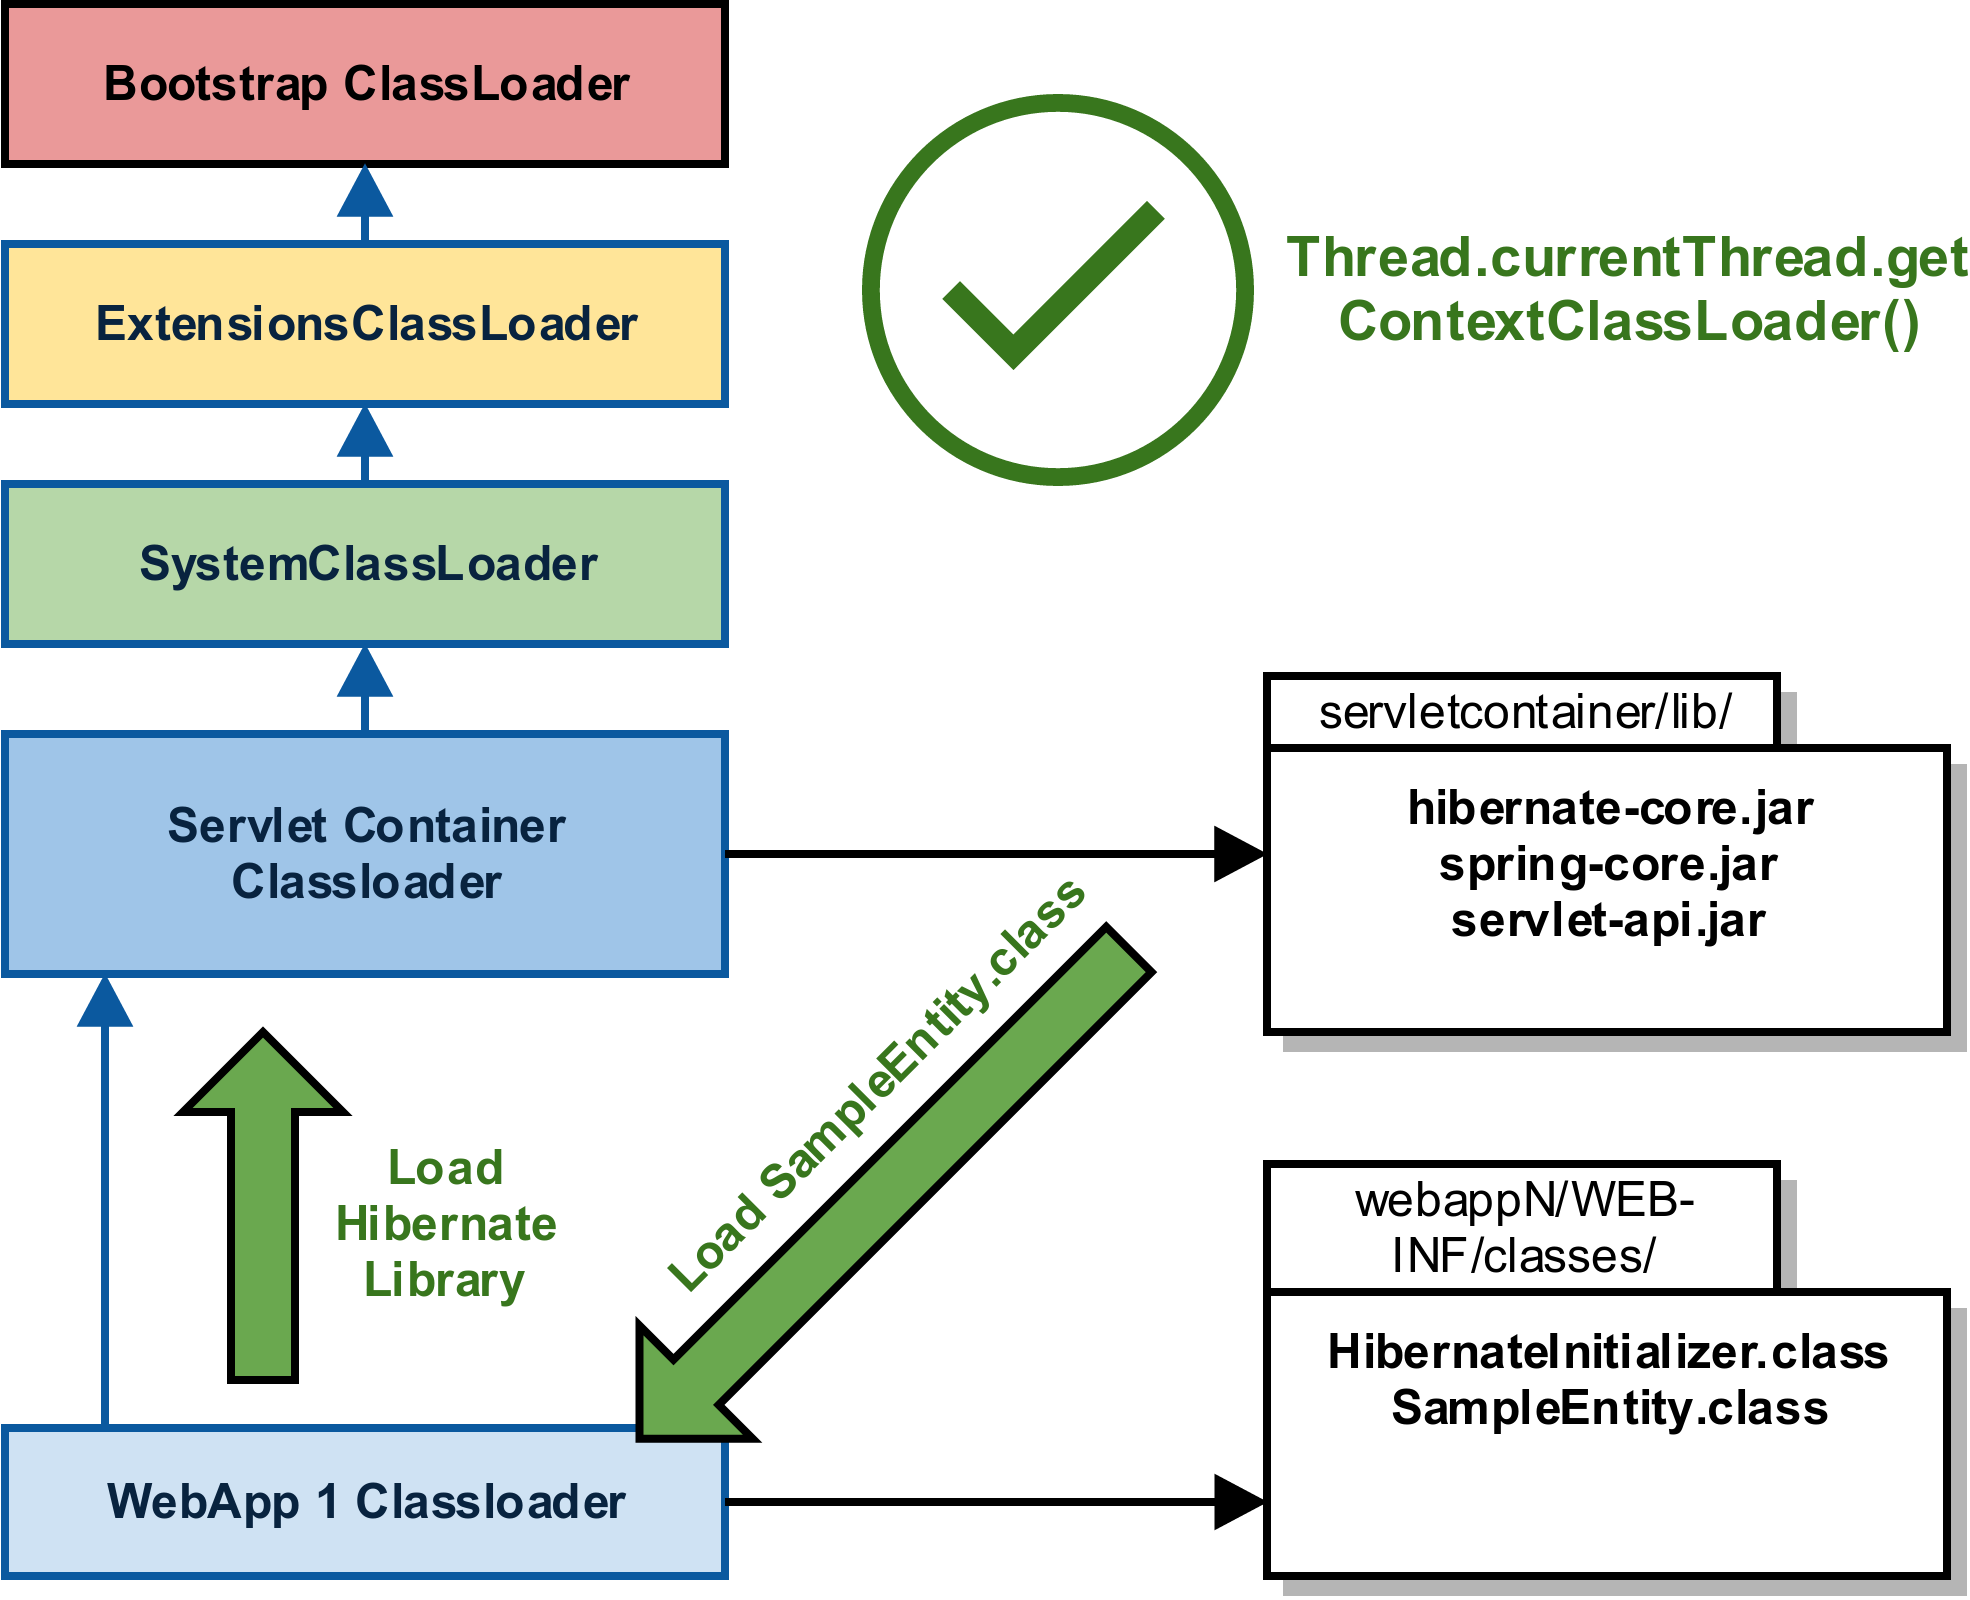
\includegraphics[scale=0.1]{assets/contextclassloader/webappclassloader-3.png} 
		\end{center}
	\end{frame}

	\begin{frame}
		Live-Demo 4: Loading the same class twice with different class loaders
	\end{frame}

	\subsection{Loading synthetic classes}

	\begin{frame}
		\frametitle{Synthetic classes}
		\begin{itemize}
			\item{Synthentic classes are ''artificial'' classes that doesn't result from your java source code}
			\item{Are created by the compiler or at runtime}
			\item{Heavy usage in the AOP world - e.g. transaktions proxy classes}
			\item{Usage in test frameworks like PowerMock}
			\item{Can be created in the class loader by definining native JVM byte code}
		\end{itemize}
	\end{frame}

	\begin{frame}
		Live-Demo 5: Creation of synthetic classes
	\end{frame}

	
	\begin{frame}
		\frametitle{End}
		
		\begin{center}
			Thank you for your attention
			\par
			Slides and sources at \href{https://github.com/fbe/classloader-vortrag}{github.com/fbe/classloader-vortrag}
		\end{center}

	\end{frame}

\end{document}

